\chapter{Pruebas y resultados}\label{chap:pruebas}

La evaluación inicial del 8 de octubre reúne 62 comprobaciones superadas en cuatro niveles: 21 sobre servicios con dependencias controladas, 15 de integración HTTP con PostgreSQL y Redis reales, 17 sobre seguridad, IA y programación de análisis, y 9 del recorrido web automatizado en Chromium. La primera corrida de servicios arroja 18 casos superados y tres defectos; corregidos, la repetición alcanza 21 de 21. Durante la construcción de la suite de 17 casos aparecen otros dos defectos, uno en la validación de cantidades en notación científica y otro en la conversión de identificadores al crear alertas, y ambos se corrigen antes de la corrida final. La regresión del 9 de octubre evalúa la versión integrada y se informa por separado en la Subsección~\ref{sec:regresion-integrada}. Las cifras de cada conjunto se mantienen separadas, y ninguna corrida automatizada reemplaza una sesión de comprensión con usuarios.

\section{Entorno, método y reproducibilidad}\label{sec:entorno-pruebas}\label{sec:validacion}

Cada caso de prueba registra identificador, requisito, entrada, resultado esperado, resultado obtenido y evidencia. Para los cálculos se utilizan carteras vacías, de una posición, de pesos iguales y de concentración desigual, con valores a ambos lados de los umbrales. Para la seguridad se prueban dos cuentas y solicitudes sin token o con token inválido. Para las señales se simula el fallo individual de proveedores y la mezcla de datos externos y locales. La medición de latencia especifica tamaño de cartera, caché, entorno y número de consultas. La comprensión se evalúa con tareas y personas independientes, registrando ayuda y errores, con carácter exploratorio (Subsección~\ref{sec:pruebas-usabilidad}); la automatización de navegador no la reemplaza.

Las ejecuciones se realizan el 8 de octubre de 2026 en macOS sobre arquitectura ARM64, con Node.js 24.11.1, PostgreSQL 18.6 y Redis 8.2.1. La API NestJS y el cliente Next.js compilan y corren en modo de producción local. Se usa una base exclusiva de evaluación, \texttt{allocia\_validation\_20261008}, y Redis en el puerto 6387. Las cuentas, tenencias e instrumentos de prueba son ficticios y la base habitual del Proyecto no se modifica.

La suite de servicios importa las clases de la API con \texttt{ts-node}, usa JWT y bcrypt reales y reemplaza repositorios, caché y respuestas HTTP externas por dobles controlados. La de integración envía solicitudes HTTP al servidor NestJS, contrasta las respuestas con los registros de PostgreSQL y consulta Redis. La de navegador opera formularios y botones del cliente Next.js con Playwright y Chrome, sin interceptar ni simular las solicitudes a la API.

Los programas están en \texttt{apps/api/tests} del repositorio de Allocia. Desde \texttt{apps/api}, con los servidores y la base de evaluación preparados, se ejecutan:
\begin{verbatim}
node -r ts-node/register tests/pfi-validation.cjs
node tests/pfi-integration.cjs
node tests/pfi-browser.cjs
\end{verbatim}
Los archivos JSON y los registros de consola de \texttt{evidence/} guardan identificadores, estados, fecha, errores y detalles de cada corrida. El registro de servicios incluye huellas SHA-256 del código probado y la carpeta \texttt{baseline/} guarda los resultados previos a las correcciones. El Anexo~\ref{annex:casos-prueba} detalla los casos; las instrucciones de preparación y ejecución acompañan a la evidencia técnica.

\section{Pruebas funcionales y de autenticación}\label{sec:pruebas-funcionales}

CP06 cubre carga, acumulación de cantidades de un mismo ticker, edición y eliminación. CP07 rechaza tickers desconocidos y cantidades cero, negativas o no numéricas. CP08 prueba los filtros de propietario en servicios con repositorios controlados. CP09 confirma la normalización del correo, bcrypt con factor 12, la aceptación de privacidad, el inicio de sesión y el rechazo de contraseña incorrecta y de correo duplicado. CP10 y CP11 ejercitan el guard con tokens ausentes, inválidos, vencidos y válidos.

La integración amplía estos casos. IT01 e IT02 registran e inician sesión por HTTP y contrastan el hash persistido. IT03 rechaza doce solicitudes a rutas privadas que combinan cuatro rutas y tres condiciones inválidas de token. IT04 ejercita los validadores HTTP e IT05 confirma que la carga y la edición quedan en PostgreSQL. IT06 usa dos cuentas: la segunda no obtiene posiciones de la primera, y sus intentos de editar o dar de baja posiciones ajenas devuelven 404 sin alterar los datos.

IT10 muestra que PostgreSQL rechaza posiciones con propietario nulo o inexistente e IT11 confirma la eliminación de una posición. IT12 exige la contraseña correcta para la baja y confirma que desaparecen la cuenta y sus posiciones; IT13, que el token anterior ya no accede a las rutas privadas ni crea posiciones mientras la otra cuenta sigue operativa. IT15 elimina la segunda cuenta de prueba sin afectar la cuenta de demostración. Estos casos aportan evidencia de autorización y eliminación en el entorno local; la concurrencia y el límite de autenticación se cubren después en SEC06 y SEC11, y la configuración remota queda fuera de esta corrida.

\section{Pruebas sobre análisis de portafolio}\label{sec:pruebas-portafolio}

CP01 confirma que la cartera vacía produce valor, HHI y número efectivo cero, sin posición dominante. CP02 usa dos unidades a precio 10 y obtiene valor 20, peso 1, HHI 10000 y número efectivo 1. CP03 usa cantidades 2, 3 y 4 y precios 10, 20 y 5. El resultado independiente esperado es:
\[
V=2\cdot10+3\cdot20+4\cdot5=100,\qquad w=(0{,}2;\,0{,}6;\,0{,}2),
\]
\[
HHI=20^2+60^2+20^2=4400,\qquad N_{\mathrm{efectivo}}=\frac{10000}{4400}\approx2{,}27.
\]
El servicio coincide con los pesos dentro de $10^{-6}$, informa HHI 4400 y presenta el número efectivo redondeado a 2,3. La agrupación regional reúne un peso 0,8 en Global y cada dimensión de composición suma 1 dentro de la tolerancia. CP04 obtiene HHI 2500 y nivel moderado para cuatro pesos iguales; CP05, HHI 1000 y nivel bajo para diez pesos iguales. IT07 contrasta los valores y el HHI devueltos por HTTP con los precios persistidos.

Estos resultados corresponden a los casos seleccionados y a su clasificación de prueba. Quedan fuera la calidad económica del catálogo, las cotizaciones actuales, las correlaciones y la capacidad predictiva; los niveles de HHI son convenciones del prototipo.

La cartera de CP03 permite mostrar qué recibe el usuario y cómo puede verificarlo. La Tabla~\ref{tab:lectura-cp03} reconstruye el cálculo con los datos que la pantalla de evidencia presenta.
\begin{table}[ht]
\centering\small
\caption{Reconstrucción del cálculo de CP03 y observaciones resultantes. Fuente: elaboración propia.}\label{tab:lectura-cp03}
\begin{tabular}{lrrrrr}\hline
\textbf{Posición} & \textbf{Cantidad} & \textbf{Precio} & \textbf{Valor} & \textbf{Peso} & \textbf{Peso$^2$ (en puntos)}\\\hline
A & 2 & 10 & 20 & 0,20 & 400\\
B & 3 & 20 & 60 & 0,60 & 3\,600\\
C & 4 & 5 & 20 & 0,20 & 400\\\hline
Total & & & 100 & 1,00 & HHI $=4\,400$\\\hline
\end{tabular}
\end{table}

Con esos valores el motor emite dos observaciones. La primera indica concentración alta, con la evidencia \enquote{HHI 4\,400; umbral de nivel alto 2\,500; posiciones efectivas 2,3} y la regla de la Tabla~\ref{tab:umbrales}. La segunda indica una posición dominante: \enquote{B pesa 60\,\%; umbral 25\,\%}. CP13 comprueba el borde de esa regla: 25\,\% no la activa y 26\,\% sí. El usuario puede repetir la multiplicación y la suma de la tabla y comprobar que la observación se desprende de sus propios datos y de un umbral declarado; no depende de un criterio oculto.

La utilidad esperada consiste en hacer visible que el resultado de la cartera depende en gran medida de B y en permitir decidir con esa información, por ejemplo si la concentración es deliberada. La observación no indica vender B ni cuánto reducirla: el HHI no mide volatilidad ni correlación, y el umbral de 25\,\% es una convención del prototipo. Que esta lectura resulte comprensible para personas sin formación financiera es la hipótesis que evalúa el protocolo del Anexo~\ref{annex:protocolo-usuarios}.

\section{Observaciones, señales y corrección de defectos}\label{sec:pruebas-observaciones}

CP12 confirma que una cartera vacía no genera observaciones. CP13 distingue el umbral de peso dominante: 25\,\% no activa la observación y 26\,\% sí. CP14 muestra que una exposición cripto de 25\,\% no activa la regla, 40\,\% produce atención y 41\,\% produce alerta. CP15, en su versión inicial, confirma que sin evidencia reciente no se generan rendimientos supuestos: los escenarios de una cartera mitad acciones y mitad cripto quedan vacíos. En la corrida del 8 de octubre este caso probaba los impactos 23,5\,\%, 6,5\,\% y $-31{,}5$\,\% de los escenarios con variaciones fijas, que la versión vigente reemplaza por escenarios con fuentes (Subsubsección~\ref{sec:reverificacion-octubre13}). Lo que se prueba es la ausencia de supuestos, no la calidad de los escenarios.

CP16 detecta al principio que \texttt{ctx-energia} omite la regla aplicada. La corrección incorpora la condición de exposición energética superior al 5\,\% y la existencia de un evento relacionado; en la repetición, todas las observaciones generadas por ese caso llevan evidencia de tipo regla. IT08 y UI04 confirman que esa regla está disponible por HTTP y se presenta al abrir la explicación. Esto prueba la trazabilidad estructural en los casos ejecutados; la comprensión requiere participantes.

CP17 simula el fallo de ambos proveedores y confirma que se mantiene el conjunto local. CP18 suministra respuestas controladas que actualizan Fear \& Greed a 22 y la dominancia BTC a 61,3, con traducción de la etiqueta. CP21 prueba la reutilización de caché y el TTL solicitado de 900 segundos. IT09 confirma la existencia del resultado y su TTL en Redis real, sin esperar 15 minutos a que expire.

CP19 reproduce el defecto inicial de etiquetar todo el conjunto como \enquote{en vivo} cuando solo un proveedor responde; la corrección introduce procedencia por componente y estado global mixto. CP20 reproduce la aceptación de Fear \& Greed 999, que la validación de rango ahora rechaza conservando el respaldo. Ambos casos pasan después del cambio.

En IT08 responden los proveedores reales Alternative.me y CoinGecko. El registro guarda las fechas informadas para Fear \& Greed y dominancia BTC y, por separado, las fechas de consulta. El contexto geopolítico, el TVL y los mercados de predicción siguen identificados como demostración. La corrida prueba una conexión efectiva en ese momento, no la disponibilidad continua ni la autenticidad histórica de los ejemplos locales.

\section{Recorrido web y rendimiento local}\label{sec:pruebas-integracion}

Los casos UI01 a UI09 corren el 8 de octubre sobre la interfaz web de ese momento; la Subsubsección~\ref{sec:reverificacion-octubre13} los repite sobre la interfaz vigente. UI01 confirma que una ruta privada redirige al acceso. UI02 registra una cuenta y obtiene una cartera vacía. UI03 carga AAPL, BTC y XLE, edita una cantidad y confirma la persistencia tras recargar. UI04 abre el análisis, despliega la regla y la fuente de energía y cambia de escenario; ese selector fue reemplazado después por escenarios con fuentes. UI05 confirma que no hay desborde horizontal a 390 píxeles, una observación que corresponde a la web adaptable y no a la aplicación nativa.

UI06 elimina una posición desde la pantalla. UI07 cierra sesión, provoca un error de contraseña y vuelve a ingresar. UI08 confirma la baja, el cierre de sesión y el rechazo de un intento posterior de inicio de sesión. UI09 registra que no hubo errores JavaScript durante el recorrido. Las capturas y las respuestas HTTP se guardan con el registro del navegador. La Figura~\ref{fig:baja-web-validada} muestra la confirmación de baja en la interfaz vigente, con datos de prueba.

\begin{figure}[ht]
\centering
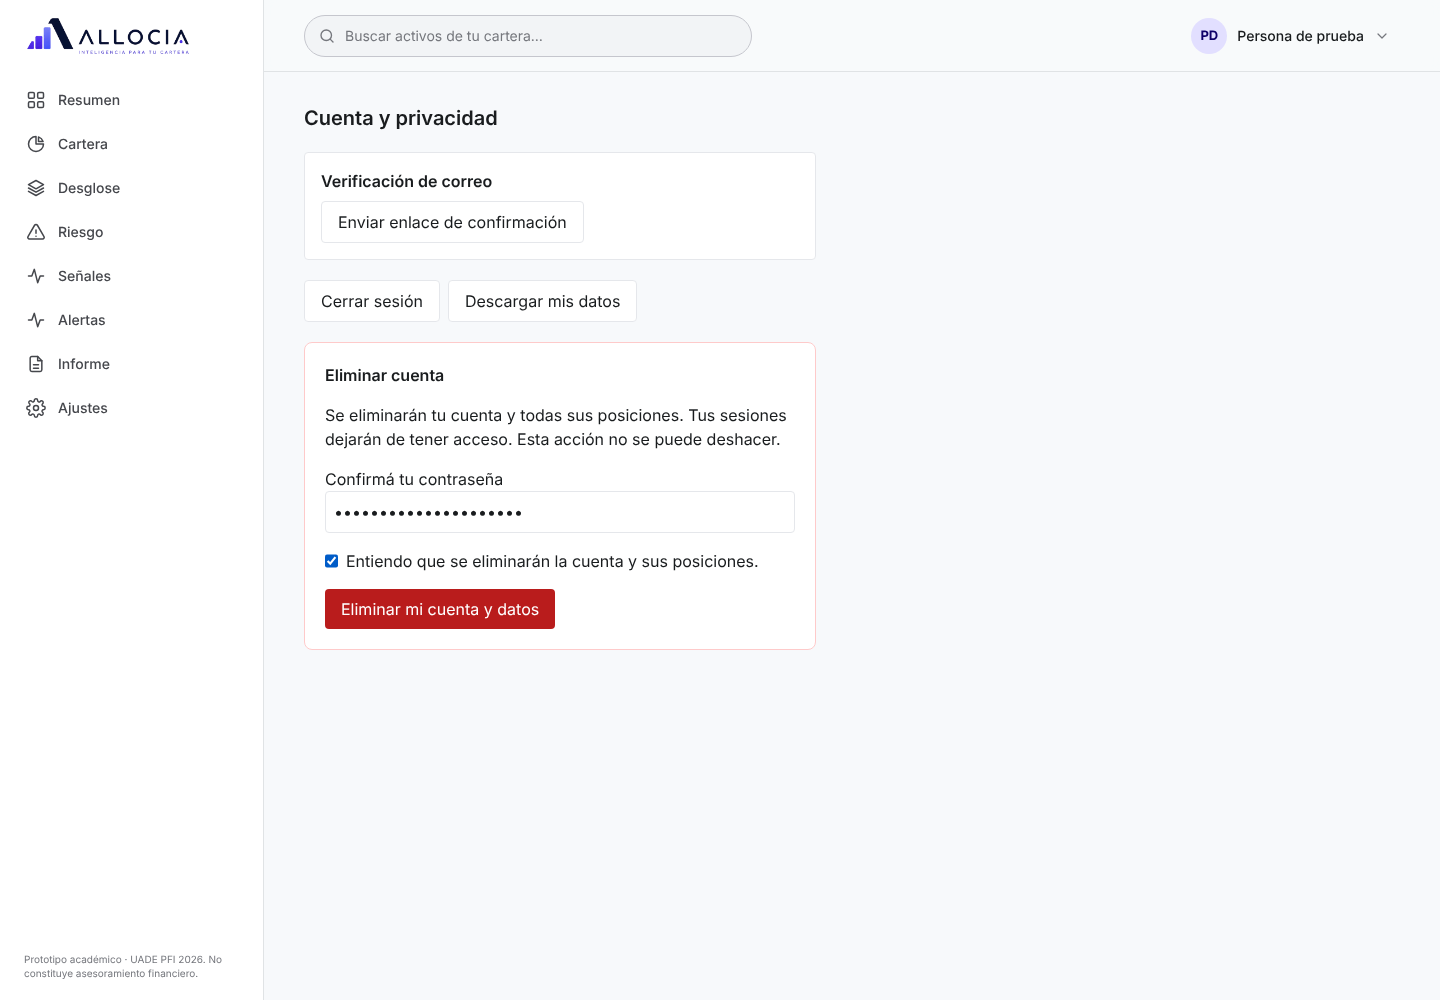
\includegraphics[width=0.95\textwidth]{figures/baja_web_reverificada.png}
\caption{Confirmación de baja en el cliente web. Fuente: captura de la reverificación del 13 de octubre de 2026.}\label{fig:baja-web-validada}
\end{figure}

IT14 usa 100 posiciones sintéticas persistidas y realiza 30 consultas secuenciales a cada endpoint, después de calentamiento. Se mide el tiempo transcurrido desde el cliente HTTP hasta completar la lectura JSON. El percentil 95 se calcula por rango más cercano, en la observación 29 de 30 ordenadas: 2,26 ms para \texttt{/analysis} y 2,89 ms para \texttt{/observations}. Ambos cumplen el umbral local de dos segundos de RNF3 en estas condiciones.

La medición incluye HTTP de bucle local, autorización, consulta a PostgreSQL y, cuando corresponde, Redis. Excluye la latencia de proveedores porque la caché está caliente, el renderizado del navegador, la red remota y la concurrencia; el resultado describe el entorno local y no el despliegue público. La revisión estática TypeScript del cliente móvil termina sin errores y Expo genera los paquetes JavaScript de iOS y Android, lo que cubre compilación y empaquetado pero deja fuera la recepción de notificaciones en dispositivos físicos y las credenciales APNs/FCM.

\section{Seguridad, IA y análisis programados}\label{sec:pruebas-produccion}

La suite adicional ejecuta 17 casos sobre la API HTTP, PostgreSQL y Redis aislados. SEC01 exige una contraseña de doce caracteres y la aceptación de la política. SEC02 confirma que el cliente web recibe una cookie \texttt{HttpOnly} con \texttt{SameSite=Strict} y no el token en el cuerpo. SEC03 rechaza mutaciones con cookie sin origen o con origen ajeno. SEC04 confirma en PostgreSQL que las cantidades se almacenan como texto cifrado AES-256-GCM, que dos cifrados del mismo valor difieren y que una etiqueta alterada no se descifra. SEC05 prueba el aislamiento entre propietarios y SEC06 ejecuta ocho acumulaciones concurrentes sobre el mismo ticker sin perder actualizaciones. SEC07 rechaza campos adicionales, cantidades excesivas y más de ocho decimales. SEC08 revoca en el servidor el token y la cookie al cerrar sesión, y SEC09 revisa las cabeceras de seguridad, la ausencia de caché y el identificador de solicitud.

AI01 acepta una salida sintética con una cita literal y rechaza identificadores, citas o escenarios sin respaldo en el conjunto suministrado. AI02 descarta noticias antiguas, futuras o con URL no HTTPS y elimina etiquetas HTML. AI03 confirma que, sin cotización, no se llama al modelo y se devuelve \enquote{datos insuficientes} sin escenarios. La prueba usa dobles y no envía solicitudes a Anthropic: ejercita el control local que precede y sigue a esa llamada.

SCH01 cubre sesiones con cambio de horario estacional, un cierre anticipado y dos cortes diarios de cripto. SCH02 ejecuta dos veces el mismo slot: una clave única y un bloqueo de PostgreSQL producen un solo informe y una sola alerta para la cuenta que posee el ticker, y el snapshot público enviado al analizador no contiene cantidad ni propietario. SCH03 confirma que otra cuenta no puede marcar la alerta como leída y que el titular puede retirar su consentimiento. SEC10 muestra que la baja elimina posiciones, alertas y dispositivos; SEC11 obtiene 429 y \texttt{Retry-After} al superar el límite de autenticación.

La auditoría de dependencias productivas de API y web termina sin vulnerabilidades conocidas por el registro usado. La del proyecto móvil mantiene avisos altos en herramientas transitivas de Expo/Metro sin una versión corregida compatible, y la compilación no los remedia. El verificador de configuración impide habilitar el despliegue cuando faltan secretos, remitente, orígenes web, calendario o universo de instrumentos; la presencia de estos parámetros es condición necesaria, no prueba de cobertura global, disponibilidad ni seguridad productiva.

\section{Regresión integrada y proveedores reales}\label{sec:regresion-integrada}

El 9 de octubre se prueba la revisión \texttt{dd2d127} del repositorio de Allocia, integrada con el nuevo cliente web. En una base aislada se repiten con éxito 21 casos de servicios, 15 de integración y 17 de seguridad, IA y programación, y se agregan tres pruebas de publicación y correo, siete de utilidades web y dos recorridos de navegador sobre la compilación productiva. Estas unidades tienen alcances distintos y se informan por separado. La API y la web compilan; el cliente móvil supera TypeScript y la exportación de paquetes iOS y Android, y los dos trabajos de integración continua de esa revisión terminan sin fallos.

El primer recorrido web cubre registro, gestión de posiciones, edición durante una indisponibilidad de cotización, alertas, exportación, revocación al salir y baja. El segundo cubre solicitud de correo, confirmación de dirección, recuperación y acceso con la contraseña nueva. La API y PostgreSQL son reales en ambos; el transporte de correo del segundo se reemplaza por un doble controlado, de modo que prueba la recuperación dentro del sistema y no la entrega externa, que se trata en la Subsección~\ref{sec:validacion-publicada} con Resend y una casilla real.

Los tokens de correo se almacenan como hashes y su copia temporal para envío se cifra con autenticación. Las pruebas cubren caducidad, propósito, uso único, consumo concurrente, respuestas genéricas, espera entre solicitudes e idempotencia de reintentos; la recuperación invalida las sesiones previas. En esa etapa la clave de Resend responde a una consulta de administración y el remitente todavía no está habilitado; la prueba posterior usa el dominio propio verificado de Allocia.

Se ejecutan además dos análisis reales, uno para AAPL y otro para BTC, con Anthropic y el modelo configurado \texttt{claude-sonnet-5-5}. Cada snapshot reúne 24 fuentes y la salida supera la validación estructural con seis hechos citados y tres escenarios. Las cotizaciones de Finnhub y CoinGecko responden correctamente. Las dos solicitudes consumen en total 17\,048 tokens de entrada y 3\,514 de salida, sin consultar tenencias personales ni enviar notificaciones. La coincidencia literal de citas y la validez del esquema son controles de forma: no prueban corrección semántica, calidad financiera ni ausencia de alucinaciones.

La prueba de cobertura obtiene una cotización válida para GGAL en su mercado estadounidense; SAP.DE, 7203.T, 0700.HK, BARC.L y GGAL.BA responden HTTP 403 con la credencial usada. Con esa credencial la cobertura regional queda incompleta, y la configuración del calendario tampoco prueba acceso licenciado a las cotizaciones de cada mercado.

Una copia cifrada de la base publicada en Railway se restaura en un entorno separado. El ensayo de migración conserva las cantidades de 23 posiciones, confirma el cifrado y el propietario obligatorio y revisa la cadena y la identidad del certificado de PostgreSQL remoto, sin modificar la base publicada ni reproducir un incidente real. La migración de correo se ensaya primero en la base de pruebas; la prueba posterior sobre el servicio publicado usa sus tablas de cuenta, tokens y envío y recorre el flujo real descrito en la Subsección~\ref{sec:validacion-publicada}.

Los registros técnicos se guardan en un paquete de evidencia saneado en el repositorio del Proyecto y los programas de ejecución se versionan en el repositorio de la aplicación. Las mediciones de latencia anteriores corresponden a la versión del 8 de octubre y no al nuevo cliente ni a los proveedores remotos.


\section{Validación del servicio publicado y cuenta compartida}\label{sec:validacion-publicada}

La evaluación se amplía el 9 de octubre de 2026 con el servicio publicado en \url{https://allocia.com.ar}. El cliente web corre en Vercel; la API, el proceso de análisis y PostgreSQL se alojan en Railway. Web y móvil usan la misma API y base de datos: la web reenvía solicitudes autenticadas desde su servidor y el móvil usa un token de acceso, sin carteras independientes que deban copiarse entre plataformas. Las pruebas emplean cuentas temporales cuyos datos se eliminan al finalizar.

La activación remota registra 17 comprobaciones superadas: cuenta, carga y edición de posiciones, búsqueda externa e importación de una criptomoneda respaldada por cotización, valuación de acciones y cripto, aislamiento de lectura y escritura, solicitud deduplicada de análisis y procesamiento de informes por el trabajador. Otra corrida confirma que las alertas internas solo están disponibles para su propietario. Estas pruebas se disparan con una solicitud manual, no con un corte automático de apertura o cierre de mercado.

El remitente de Allocia usa un dominio propio verificado. El flujo remoto supera 15 comprobaciones que incluyen solicitud, consumo del enlace, rechazo de reutilización, cambio de contraseña, revocación de la sesión previa, rechazo de la contraseña anterior e ingreso con la nueva. Resend informa la entrega de los dos mensajes, \enquote{Confirmá tu correo} y \enquote{Recuperá tu acceso}, y el destinatario autorizado confirma que ambos llegan a Recibidos. A diferencia del doble de transporte usado antes, esta evidencia cubre envío y recepción en una casilla real, aunque no la entregabilidad a todos los proveedores de correo ni tiempos garantizados de recepción.

\subsection{Persistencia entre web y móvil}\label{sec:persistencia-web-movil}

La prueba remota de cuenta compartida registra 18 comprobaciones superadas. Una cuenta creada desde la web inicia sesión con el cliente HTTP real de la aplicación móvil y obtiene el mismo identificador. La posición creada desde ese cliente aparece en la web y la edición web se observa desde el móvil; las preferencias de alertas se conservan en ambos sentidos. Una segunda cuenta no obtiene esas posiciones ni puede editarlas o eliminarlas, la baja desde la web impide usar el token móvil previo y la exportación consulta las mismas posiciones persistidas.

El recorrido de navegador local complementa ese ensayo: al recuperar el foco, la web muestra una modificación hecha desde el cliente móvil sin perder el texto de un formulario en curso. Las pantallas consultan los datos cada 30 segundos mientras están visibles y al volver al primer plano. Se trata de una actualización periódica que requiere conectividad, no de una sincronización instantánea por transmisión continua, y las cotizaciones del proveedor siguen sin ser precios de latencia garantizada.

El cliente HTTP móvil corre en el entorno de pruebas, sin emular una interacción física en iOS o Android. La igualdad de las listas de informes de las cuentas temporales no informa sobre la generación de análisis cuando la lista está vacía; esa evidencia proviene de las corridas específicas de IA y del proceso de análisis.

\subsection{Cobertura de datos e integración del protocolo de análisis}

La consulta del catálogo obtiene cotizaciones para sus 34 instrumentos en el momento registrado. El resultado corresponde a ese universo, no a todas las acciones, bolsas o criptomonedas existentes. La búsqueda externa permite incorporar instrumentos adicionales cuando el proveedor devuelve una cotización comprobable. Los rechazos de acceso de otros mercados y de históricos bursátiles se registran como limitaciones: encontrar un símbolo no significa disponer de todos sus datos.

El protocolo de análisis estructurado incorpora indicadores diarios deterministas, seguimiento entre informes y un veredicto con estados declarados de disponibilidad. Entre los indicadores se incluyen medias móviles, el RSI, el MACD, las bandas de Bollinger y variaciones calculadas sobre la serie disponible, definidos en la Subsubsección~\ref{subsubsec:indicadores-tecnicos}. Se controlan el tamaño de muestra y la antigüedad, y las series faltantes no se reemplazan por cifras generadas por el modelo. Las pruebas de investigación y cotizaciones reúnen 12 casos superados, incluidos validación de fechas, datos insuficientes y coherencia de los cálculos macroeconómicos.

El contexto macroeconómico agrega cuatro series oficiales de FRED: tasa efectiva de fondos federales, rendimientos del Tesoro estadounidense a dos y diez años e índice de precios al consumidor desestacionalizado \parencite{FREDDFF,FREDCPI}. Cada observación guarda fecha, unidad y fuente. La inflación interanual se calcula contra el mismo mes del año anterior y el diferencial de rendimientos exige observaciones de igual fecha. Las cuatro series se recuperan desde Railway; su cobertura es estadounidense y su frecuencia de publicación no es tiempo real.

Una nueva solicitud real para BTC con Anthropic y la versión \texttt{allocia-evidence-5} incorpora ese contexto, obtiene cuatro hechos citados y tres escenarios y supera los controles de estructura y evidencia. Los apartados sin respaldo se marcan como no disponibles: no se atribuyen probabilidades calibradas, puntajes de inversión, precios de entrada, precios objetivo ni niveles de salida ante pérdidas (\textit{stops}). El control de citas reduce una clase de errores; la exactitud semántica, la capacidad predictiva y la validez de una estrategia financiera completa quedan fuera de lo probado.

Una consulta a las señales del servicio publicado, realizada el 22 de octubre con la cuenta de demostración, devuelve el conjunto con origen \enquote{fuentes externas} y procedencia por componente: Fear \& Greed de Alternative.me (68), dominancia de BTC de CoinGecko (59,5\,\%), TVL de DefiLlama (89\,912 millones de dólares), cinco mercados de Polymarket con su precio implícito y seis noticias de Finnhub, cada uno con la fecha del dato y la de consulta. En esa consulta el índice GPR figuraba como no disponible. El 23 de octubre, tras desplegar la integración de la planilla diaria de Caldara e Iacoviello, una nueva consulta devuelve GPR 176 (nivel elevado, tendencia estable) con fecha del dato 19 de octubre y fuente identificada; desde el despliegue siguiente, la regla \texttt{ctx-gpr} y las demás reglas apoyadas en señales externas quedan activas en producción con datos reales. Las respuestas se conservan en \texttt{evidence/2026-10-22-senales-produccion} y \texttt{evidence/2026-10-23-gpr-produccion}.

\subsection{Regresión, publicación, notificaciones y registro}

La suite de seguridad e integración ampliada supera 21 comprobaciones con HTTP, PostgreSQL y Redis reales aislados; las fuentes y el modelo se simulan en los casos de programación y validación de citas. La integración continua de las revisiones \texttt{8768e53} y \texttt{015e7b6} termina sin fallos: la primera corresponde a la ampliación macroeconómica y la segunda incluye la prueba cruzada web/móvil. La web publicada se revisa en Vercel y la API responde con el identificador de su revisión desplegada. Los cambios exclusivos de clientes no requieren una revisión nueva de la API.

Las revisiones TypeScript de ambos clientes y el empaquetado JavaScript de iOS y Android terminan correctamente. La web actualiza informes y alertas; el móvil incorpora la exportación de datos personales con el menú nativo para compartir texto JSON, cuyo funcionamiento en un teléfono se confirma en la prueba física de la Subsubsección~\ref{sec:confirmacion-fisica}. La matriz de paridad registra las diferencias entre clientes: el navegador no recibe notificaciones push y la web ofrece algunas vistas y exportaciones adicionales.

Se configuran APNs para iOS, FCM v1 para Android y la autenticación de envíos en Expo, y se confirma el acceso del token al proyecto y la activación en API y proceso de análisis. El registro de esa prueba contiene cero dispositivos, por lo que la entrega física se documenta más adelante con los instaladores y la recepción en iPhone de la Subsubsección~\ref{sec:revision-octubre10}. Las alertas internas probadas son distintas de las notificaciones push recibidas.

El repositorio del Proyecto incorpora un manifiesto saneado con fechas, revisiones, resultados y huellas SHA-256 de los registros de origen. El archivo \path{evidence/2026-10-09-actualizacion.json} identifica cada evidencia sin incluir claves, tokens de sesión ni datos de carteras personales. Los programas de prueba se guardan en el repositorio de Allocia, incluidos \path{apps/web/e2e/shared-account.spec.ts} y \path{scripts/shared-account-smoke.cjs}. Las cifras de cada ensayo mantienen su unidad, sea casos, recorridos o comprobaciones, y no se suman en un porcentaje de calidad o de cumplimiento.

\section{Comprensión con usuarios: resultados}\label{sec:pruebas-usabilidad}

Entre el 21 y el 23 de octubre de 2026 se aplicó el protocolo del Anexo~\ref{annex:protocolo-usuarios} a cinco participantes ajenos al equipo y al tutor: tres inversores activos (U01 a U03), una persona de seguimiento ocasional (U04) y una que evalúa comenzar a invertir (U05). Tres sesiones fueron presenciales y dos por videollamada; los dispositivos cubrieron la web en notebook y en teléfono y las aplicaciones Android e iOS. Cada participante usó una cuenta ficticia con posiciones de ejemplo (2 AAPL, 0,1 BTC y 100 XLE). El moderador registró inicio, fin, resultado, errores, ayuda y respuesta literal de cada tarea; el registro completo está en \texttt{evidence/2026-10-sesiones-usuarios} y se resume en el Anexo~\ref{annex:protocolo-usuarios}.

Dos condiciones del servicio publicado obligaron a adaptar el protocolo. La regla de exposición energética no se activó, porque en producción no se publican los eventos locales de demostración; la tarea 3 se aplicó sobre la observación de posición dominante, que BTC activa con un peso cercano al 51\,\%, y el criterio de comprensión pasó a ser identificar sin ayuda la condición del 25\,\% y que el cálculo proviene de la propia cartera. Los escenarios con fuentes no estaban disponibles para esos activos durante las sesiones, de modo que esa parte de la tarea 4 no se evaluó y se registró aparte. La Tabla~\ref{tab:sesiones-resultados} resume los resultados por tarea.

\begin{table}[ht]
\centering\small\renewcommand{\arraystretch}{1.15}
\caption{Resultados de las sesiones por tarea (cinco participantes). Fuente: elaboración propia.}\label{tab:sesiones-resultados}
\begin{tabular}{>{\raggedright\arraybackslash}p{5.4cm}cccc}\hline
\textbf{Tarea} & \textbf{Sin ayuda} & \textbf{Con ayuda} & \textbf{No completada} & \textbf{Mediana (min)}\\\hline
1. Crear cuenta, cargar y editar posiciones & 2 & 3 & 0 & 7,5\\
2. Mayor posición y concentración & 3 & 2 & 0 & 3,4\\
3. Explicar una observación (criterio) & 2 & 2 & 1 & 4,6\\
4. Fuentes, fechas y escenarios & 1 & 2 & 2 & 6,3\\
5. Eliminar posición y dar de baja la cuenta & 2 & 2 & 1 & 6,0\\\hline
\end{tabular}
\end{table}

Los cinco participantes completaron la carga y la edición de posiciones, aunque solo dos sin ayuda: U03 volvió a agregar AAPL en lugar de editarlo, U04 no encontró la edición en la pantalla del teléfono y U05 ingresó un monto en dinero donde se piden unidades. La sesión más corta duró 23 minutos (U01) y la más larga 50 (U05). En la tarea 2, los tres inversores activos identificaron a BTC como la mayor posición en menos de dos minutos y describieron la concentración con sus palabras (\enquote{con tres activos igual podés estar muy concentrado; no depende del número de renglones}, U03). U04 respondió primero con el porcentaje del sector energía y U05 confundió el valor total con el de BTC y el porcentaje con una ganancia; ninguno de los dos explicó el índice, pero ambos entendieron que la cartera estaba poco repartida.

La tarea 3 es la que mide la hipótesis del MVP. Dos participantes identificaron sin ayuda la condición y su origen: \enquote{la regla salta arriba de 25\,\% en un activo, y el porcentaje se calcula con la cartera que armé; esto no es una orden de vender} (U03). U02 y U04 leyeron la observación como una alerta por movimiento de precio o por una noticia sobre bitcoin; cuando el moderador pidió abrir la evidencia y leer el umbral aplicado, ambos corrigieron la lectura. U05 no logró relacionar el umbral con el peso de BTC y preguntó si el 25\,\% era \enquote{lo que tengo que vender o el máximo que puedo comprar}. El criterio exploratorio de cuatro de cinco sin ayuda no se alcanzó: el resultado es dos de cinco. En la tarea 4 todos ubicaron el proveedor de al menos un indicador, pero la diferencia entre fecha del dato y fecha de consulta fue el obstáculo principal: cuatro de los cinco la confundieron al menos una vez y dos no llegaron a explicarla. En la tarea 5 los cinco comprobaron que BTC no reaparecía al volver a entrar; dos confundieron cerrar sesión con eliminar la cuenta y U05 prefirió no confirmar la baja, decisión que se respetó y no se contó como eliminación.

Las respuestas de cierre coinciden con lo observado. Lo más confuso fueron las fechas (U01, U04, U05) y el vocabulario de la pantalla de riesgo (U04, U05); U02 señaló que \enquote{la advertencia parecía de mercado y era de mi cartera}. Lo más valorado fue ver el motivo del aviso (U01, U03) y la facilidad de carga (U02, U04, U05). La Tabla~\ref{tab:sesiones-cambios} traduce cada hallazgo en un cambio concreto. Los ocho cambios se implementaron en los dos clientes y se desplegaron el 23 de octubre (revisión \texttt{a0d28c0} de Allocia): la web en \url{https://allocia.com.ar} y la aplicación móvil en nuevos instaladores internos. La repetición de la evaluación con los cambios aplicados no forma parte del Proyecto y se plantea como trabajo futuro.

\begin{table}[ht]
\centering\small\renewcommand{\arraystretch}{1.15}
\caption{Hallazgos de las sesiones y cambios derivados. Fuente: elaboración propia.}\label{tab:sesiones-cambios}
\begin{tabular}{>{\raggedright\arraybackslash}p{4.6cm}>{\raggedright\arraybackslash}p{6.4cm}>{\raggedright\arraybackslash}p{2.6cm}}\hline
\textbf{Hallazgo (participantes)} & \textbf{Cambio} & \textbf{Estado}\\\hline
Fecha del dato y fecha de consulta se confunden (U01, U03, U04, U05) & Rótulos explícitos \enquote{Dato del} y \enquote{Consultado el}, con ayuda contextual, en web y móvil & Implementado\\
La observación de cartera se lee como noticia de mercado (U02, U04) & Etiqueta y color distintos para \enquote{Sobre tu cartera} y \enquote{Contexto externo}; la regla visible en la tarjeta, no solo en el desplegable & Implementado\\
El índice de concentración no se entiende sin formación (U04, U05) & Explicación en lenguaje llano con ejemplo junto al indicador y entrada en el glosario & Implementado\\
Editar se confunde con volver a agregar; acceso poco visible en el teléfono (U03, U04, U05) & Botón \enquote{Editar} en cada posición; al cargar un ticker existente, ofrecer editar en lugar de sumar la cantidad & Implementado\\
Cantidad interpretada como dinero (U05) & Rótulo \enquote{cantidad en unidades} y ejemplo en el campo & Implementado\\
Cerrar sesión se confunde con eliminar la cuenta; la baja se busca en Cartera (U02, U04) & Separar ambas acciones en Cuenta, con aviso para exportar antes de eliminar (pedido de U03) & Implementado\\
No queda claro que no hay escenarios recientes (U02, U03) & Mensaje explícito y botón para solicitar el análisis desde la misma pantalla & Implementado\\
Confirmación de guardado demasiado breve (U02) & Confirmación persistente hasta la próxima acción & Implementado\\
Comparar carteras antes de guardar un cambio (U01) & Simulación de cambios sobre la composición & Trabajo futuro\\\hline
\end{tabular}
\end{table}

La hipótesis del MVP queda respaldada en parte. Los inversores activos comprenden la observación y su evidencia con poca o ninguna ayuda; las personas con seguimiento ocasional o sin experiencia necesitan un lenguaje más simple y una distinción visual entre lo que proviene de su cartera y lo que proviene del contexto. La explicación es inspeccionable, pero no es autosuficiente para quien recién empieza; RNF1 no se cumple en la evaluación realizada, y el efecto de los cambios aplicados no se volvió a medir. Los resultados describen la experiencia de cinco personas elegidas por conveniencia, con un moderador del equipo y sin generalización estadística; la clasificación de una respuesta como \enquote{sin ayuda} depende del criterio del moderador registrado en cada ficha.

\section{Síntesis y alcance de los resultados}\label{sec:resultados-pruebas}

Las 62 comprobaciones de la evaluación inicial cumplen sus condiciones: 21 de servicios, 15 de integración, 17 de seguridad, IA y programación, y 9 de navegador. La cuenta, la cartera, el cifrado, la validación de evidencia, el calendario y las alertas funcionan en los casos locales ensayados; la baja elimina los datos activos vinculados y bloquea los tokens de la cuenta eliminada.

La Tabla~\ref{tab:verificado-criterios} resume, para cada aspecto del valor atribuido al sistema, qué resultado se esperaba, cómo se probó y qué falta. La reverificación del 13 de octubre (Subsubsección~\ref{sec:reverificacion-octubre13}) repite los conjuntos de servicios, integración, seguridad y navegador y agrega pruebas web adicionales, sin modificar las conclusiones de esta sección.
\begin{table}[ht]
\caption{Qué se verificó, con qué criterio y qué falta. Fuente: elaboración propia.}\label{tab:verificado-criterios}
\centering\footnotesize\renewcommand{\arraystretch}{1.2}
\begin{tabular}{>{\raggedright\arraybackslash}p{2.6cm}>{\raggedright\arraybackslash}p{4.0cm}>{\raggedright\arraybackslash}p{4.4cm}>{\raggedright\arraybackslash}p{3.4cm}}\hline
\textbf{Aspecto} & \textbf{Resultado esperado} & \textbf{Cómo se verificó} & \textbf{Estado y límite}\\\hline
Cálculo de pesos, exposiciones y HHI & Pesos con error máximo de $10^{-6}$ frente a un cálculo independiente; HHI de 4\,400 para CP03 & CP01 a CP05 e IT07; reconstrucción manual de la Tabla~\ref{tab:lectura-cp03} & Verificado en carteras seleccionadas; no valida la calidad económica de los precios\\
Umbrales de las observaciones & Activación en el borde declarado de la Tabla~\ref{tab:umbrales}: 25\,\% no activa y 26\,\% sí; cripto 25, 40 y 41\,\% & CP04, CP05, CP13 y CP14, con valores a ambos lados de cada umbral & Verificado; los umbrales son convenciones del prototipo\\
Trazabilidad de la observación & Todas las observaciones con regla, métricas y evidencia & CP16, IT08 y UI04 & Verificado en los casos ejecutados\\
Procedencia de las señales & Fuente, fecha y condición (en vivo o demostración) por componente & CP17 a CP20, IT08 y X05, con fallos simulados y consultas reales & Verificado; sin cobertura global ni disponibilidad continua\\
Aislamiento y protección de datos & Rechazo de acceso ajeno, cantidades cifradas y baja completa & IT06, IT10 a IT13, SEC04 a SEC08 y SEC10, con dos cuentas en PostgreSQL aislado & Verificado; sin auditoría independiente\\
Informes con modelo de lenguaje & Citas literales y abstención ante datos insuficientes & AI01 a AI03 y dos ejecuciones reales (AAPL y BTC) & Verificado en estructura; no demuestra corrección semántica\\
Utilidad para el usuario & Al menos cuatro de cinco participantes identifican la causa y la fuente de una observación sin ayuda & Cinco sesiones con el protocolo del Anexo~\ref{annex:protocolo-usuarios} & Criterio no alcanzado: dos de cinco sin ayuda\\\hline
\end{tabular}
\end{table}

El total de casos no expresa cobertura de código ni porcentaje de requisitos cumplidos. La evaluación posterior cubre acceso público, cuentas compartidas, entrega real de correo, cotizaciones del catálogo, análisis reales y contexto macroeconómico. La protección de datos y la trazabilidad quedan respaldadas por los casos ejecutados, sin que esto equivalga a una auditoría de seguridad.

Quedan fuera de lo verificado la repetición de la evaluación con usuarios después de los cambios derivados, la observación del disparo previo a la apertura, las diferencias de paridad documentadas y la cobertura adicional de fuentes. Los datos históricos y en vivo no son las únicas condiciones abiertas. La latencia local cumple el criterio en su escenario medido; el desempeño remoto y la utilidad o calidad financiera no se desprenden de estas pruebas.


\section{Revisiones posteriores y reverificación}\label{sec:revisiones-posteriores}

Las revisiones de octubre amplían la evaluación inicial con nuevas funciones, pruebas físicas y una reverificación completa. Se presentan en orden cronológico; cada una conserva su fecha y su evidencia.

\subsection{Revisión integrada del 10 de octubre}\label{sec:revision-octubre10}

La revisión posterior incorpora la evidencia producida por el uso del prototipo por parte de sus autores. Se confirma la recepción push en un iPhone con una captura del aviso aportada por el usuario, y los instaladores internos de iOS y Android con biometría se generan correctamente en Expo. Esta evidencia no alcanza la recepción en Android, todas las condiciones de entrega, el funcionamiento de los sensores físicos ni una evaluación independiente de usabilidad.

Se detectan y corrigen dos defectos del pedido manual: las alertas antiguas aparecían antes que los informes recientes y la pausa de notificaciones automáticas afectaba al solicitante manual. La regresión sobre HTTP, PostgreSQL y Redis aislados reúne 22 comprobaciones superadas, con dos cuentas sobre un mismo activo, solicitudes dentro de una hora, selección del último informe, pausa de avisos ajenos e idempotencia; esta suite no envía notificaciones reales. La API publicada se prueba con una cuenta temporal, que registra una duración de sesión de 604800 segundos y luego se elimina.

La revisión técnica ejecuta, además, 20 pruebas controladas de indicadores, cotizaciones, publicación, correo, traducción y escenarios, y ocho pruebas de utilidades web, todas superadas. Los ensayos de cotizaciones cubren caducidad, agrupación de consultas, actualización manual, conservación de la fecha del proveedor y ausencia de reemplazo silencioso después de un fallo. Las pruebas de interfaz móvil cubren cancelación biométrica, bloqueo al volver del fondo, rechazo de resultados tardíos y preservación de la sesión sin red. Estos conjuntos tienen alcances distintos y se informan por separado.

Tres recorridos de navegador cubren recuperación y verificación de correo, gestión completa de cuenta y cartera, y datos compartidos entre web y cliente móvil. Pasan contra una API y una base de datos aisladas, con correo simulado; la entrega real ya se confirmó en una prueba anterior.

Una consulta desde Railway el 10 de octubre a las 20:55 UTC obtiene AAPL a 336,64 USD con fecha del 9 de octubre a las 20:00 UTC, y BTC a 83006 USD con fecha del 10 de octubre a las 20:54:43 UTC. El contraste explica que una valuación pueda cambiar sin que cambie la fecha de todas sus posiciones, sin que ello suponga acceso a streaming ni cobertura de todos los instrumentos.

Las evidencias y regresiones se guardan en el repositorio de la aplicación, distinguiendo código probado, versión desplegada y resultado físico. Las mejoras posteriores requieren instalar la nueva versión móvil.

\subsection{Preparación de la prueba física}\label{sec:preparacion-fisica}

La consulta de registros productivos del 10 de octubre muestra una ejecución previa al cierre de NYSE/Nasdaq, creada el 9 de octubre a las 19:45:19 UTC y completada a las 19:49:19 UTC con 25 informes, y los cortes de cripto del 10 de octubre a las 00:00 y 12:00 UTC, completados con nueve informes cada uno. Esta evidencia cubre programación y persistencia, no la recepción física de cada aviso. El disparo previo a la apertura no se observó.

Se incorpora el estado por activo de las solicitudes manuales en web y móvil: en espera, analizando, listo o no completado. La consulta se restringe al solicitante y a sus tenencias vigentes, sin publicar errores internos del proveedor. La regresión de seguridad e integración alcanza 23 comprobaciones superadas, y una prueba adicional cubre aislamiento, vigencia, modificación de cantidades, actualización manual, concurrencia y eliminación de la instantánea de valuación ante un fallo. Los tres recorridos completos de navegador vuelven a pasar.

Los instaladores de prueba incorporan estos cambios junto con el reintento de sesión sin red. El protocolo físico registra dispositivo, versión, biometría, retorno desde segundo plano, reconexión, actualización entre web y móvil, estado de informes, recepción push y exportación.


\subsection{Confirmación física y evolución visual}\label{sec:confirmacion-fisica}

El 10 de octubre se completan las pruebas físicas propuestas en Android e iOS con resultado correcto, según informa Mauricio Huentelaf. La confirmación corresponde a los instaladores internos Android \texttt{5197fba7} e iOS \texttt{a1f76f64}, generados desde la revisión \texttt{94d5850}. El recorrido comprende ingreso y visibilidad de contraseña, desbloqueo y cancelación biométrica, retorno desde segundo plano, apertura sin red y reconexión, modificaciones compartidas con la web, actualización de cotizaciones, estado de análisis, notificaciones y exportación. Se trata de una aceptación informada por quien desarrolló el prototipo, no de un ensayo independiente de usabilidad, y no se agregan tiempos de ejecución que no fueron informados.

Los equipos son iPhone 17 Pro Max e iPhone 14, ambos con iOS 27, y Samsung Galaxy A16 con One UI 8.5; la versión web también pasa en una MacBook Pro. En el equipo local se registra macOS 27.2 con \texttt{sw\_vers}, compilación \texttt{26B5101f}. Los modelos y las versiones móviles proceden del reporte del usuario; One UI identifica la interfaz de Samsung, sin inferir la versión base de Android, y no se informó la versión del navegador.

Esta evidencia completa el protocolo físico para esos instaladores. Quedan fuera la permanencia durante siete días completos, la cobertura universal de proveedores y la recepción de cada corte automático; la evaluación con participantes se presenta en la Subsección~\ref{sec:pruebas-usabilidad}.

La mejora siguiente incorpora logos de activos en Cartera web y móvil, con el símbolo legible. La API consulta metadatos de Finnhub y CoinGecko y admite imágenes raster desde dominios restringidos, con límites de tamaño y tiempo; las claves quedan en el servidor. Si no existe logo o falla la descarga se muestra la abreviatura, sin asignar imágenes de otro activo. Las pruebas automatizadas cubren caché, concurrencia, ausencia de reenvío de credenciales y rechazo de direcciones no admitidas y de formatos no permitidos. Esta evolución visual es posterior a la aceptación física y se incluye en los nuevos instaladores descritos al final de la Subsubsección~\ref{sec:refinamiento-legibilidad}.

\subsection{Refinamiento de legibilidad y estados de interacción}\label{sec:refinamiento-legibilidad}

Tras la aceptación física se revisa la presentación de Cartera y de los informes en web y móvil. Cada activo dispone de bloques rotulados para cantidad, precio por unidad y valor de la posición en USD, con una jerarquía tipográfica que destaca el valor. La fecha del precio sigue visible; la fuente, la fecha de consulta y la explicación de posibles demoras se agrupan en un desplegable. Los cálculos no cambian y la fecha de consulta no se presenta como una cotización nueva. En móvil se prioriza el total y se permite abrir el formulario de alta cuando la cartera ya contiene activos; en web se mantienen búsqueda y ordenamiento.

Los estados de carga se distinguen de una cartera o lista de informes vacía. Se incorporan estructuras de carga discretas, indicación de actualización y acciones de reintento en las pantallas principales. Los botones principales ganan área de interacción y se admite el ajuste del texto del sistema. La vista de informes separa resumen, escenarios condicionales, limitaciones y fuentes. Un glosario desplegable explica RSI, SMA, MACD y volatilidad cuando aparecen en el resumen, sin alterar el texto original ni añadir pronósticos o probabilidades. El precio usado al generar un informe se identifica como tal, separado de la cotización consultable en Cartera.

La prueba automatizada recorre registro, edición de posiciones, continuidad entre clientes y estados de carga y error. La revisión de diseño web usa anchos de 320, 390, 768 y 1280 píxeles, además de texto al 200\%, sin desbordamiento horizontal en el recorrido evaluado. Para revisar informes y fallos se usan respuestas controladas, identificadas como datos de prueba. La revisión TypeScript y el empaquetado de JavaScript para iOS y Android completan estas pruebas. La aceptación de la Subsubsección~\ref{sec:confirmacion-fisica} corresponde a los instaladores previos, de modo que la prueba física de esta presentación se informa a continuación; no cuenta con certificación de accesibilidad ni con validación con usuarios de todos los grupos etarios.

El 10 de octubre se generan los instaladores internos Android \texttt{a38311fb} e iOS \texttt{d5537a7d}, desde la revisión \texttt{e068feb}, con logos y refinamiento de legibilidad. Ambos artefactos quedan disponibles para descarga; la prueba previa cubre la API \texttt{94a36f6}, y se corrige una referencia obsoleta que había detenido el primer intento. La prueba física informada después por Mauricio Huentelaf pasa en logos, jerarquía de cantidades y precios, formulario de alta, estados de carga y reintento, y presentación y ayuda contextual de los informes, con lo que se completa la aceptación física de esta revisión. El resultado corresponde a ese reporte, sin mediciones por caso, y es distinto de las sesiones independientes de usabilidad.

\clearpage
\subsection{Validación de oportunidades sobre activos no poseídos}\label{sec:pruebas-oportunidades}

La ampliación de la Subsección~\ref{sec:oportunidades} se prueba con datos sintéticos identificados. Las pruebas de evidencia rechazan informes antiguos, citas inválidas, fuentes futuras, escenarios de baja, datos insuficientes y noticias cripto sin relación específica con el token; la salida válida conserva condición y fuente, sin porcentaje de probabilidad. La integración con PostgreSQL aislado cubre migración, aislamiento entre listas de seguimiento, deduplicación manual, separación de alertas de cartera y de oportunidad, consentimiento independiente, cancelación de avisos pendientes, reemplazo por un informe más reciente y eliminación en cascada.

El transporte push simulado revisa el símbolo y el texto condicional de la oportunidad. La prueba de navegador ejercita las preferencias y el seguimiento contra la API, y usa búsqueda e informes controlados para revisar fuentes, separación de vistas y anchos de 320, 390 y 1280 píxeles. Estos ensayos no miden precisión predictiva ni rentabilidad. La aceptación física informada para los instaladores anteriores se mantiene; la nueva clase de alerta requiere probarse en el instalador que la incorpore.

La prueba publicada usa una cuenta temporal y confirma la migración operativa, el acceso autenticado, el seguimiento de Tesla sin tenencias, las preferencias independientes y su exportación, y la misma lista desde web y API móvil. La cuenta se elimina al finalizar. En esta prueba no se dispara un análisis con el modelo ni un push real; esos alcances corresponden a las pruebas con dependencias controladas.

Los instaladores Android \texttt{8a312f48} e iOS \texttt{3e5deb95}, de la revisión \texttt{d58c665}, se generan correctamente y sus descargas se confirman. La API publicada corresponde a \texttt{2174898}, con un ajuste compatible para evitar coincidencias ambiguas de nombres cripto. Los controles de integración continua de ambas revisiones terminan sin fallos. Estos resultados cubren distribución y prueba técnica, no la recepción física de la nueva notificación.

La revisión posterior detecta que el selector móvil regresaba a Mi cartera al desmontar la pantalla de Alertas. Se corrige conservando la vista elegida en la navegación y en el almacenamiento local por cuenta. Las pruebas automatizadas cubren restauración al reiniciar, separación entre cuentas, prioridad de una selección nueva frente a una lectura tardía y orden de guardado. La corrección no toca el consentimiento de notificaciones persistido en el servidor y no se probó en un equipo físico, porque exige instalar una versión que la incluya.

\subsection{Reverificación del 13 de octubre}\label{sec:reverificacion-octubre13}

La reverificación repite los casos de las Subsecciones~\ref{sec:pruebas-funcionales} a~\ref{sec:pruebas-produccion} sobre una base de datos y un Redis aislados, creados desde cero. Pasan los 21 casos de servicios, las 15 pruebas de integración HTTP, las 23 comprobaciones de seguridad, IA y programación y las 33 pruebas unitarias adicionales. El recorrido de navegador se actualiza a la interfaz vigente y reúne 21 comprobaciones, UI01 a UI09, UI04b y X01 a X11, también superadas. Cada conjunto mantiene su unidad y se informa por separado. El Anexo~\ref{annex:casos-prueba} detalla los casos.

Se detecta y corrige un defecto en la baja de cuenta. Ante una contraseña incorrecta la API responde 401, como corresponde, pero el cliente web lo trataba como sesión vencida: eliminaba la cookie, redirigía al ingreso y no mostraba el motivo. La cuenta no se eliminaba ni quedaba información expuesta, pero la persona perdía la sesión con un mensaje engañoso. La corrección distingue la contraseña incorrecta de una sesión vencida sin tocar la API ni su contrato. Dos pruebas nuevas, una unitaria y un recorrido de navegador, fallan sin la corrección y pasan con ella; la baja permite ahora reintentar con la contraseña correcta.

La suite Playwright, ejecutada sin ajustes, pasa 4 de 26 pruebas: las restantes buscan textos y selectores de una interfaz anterior y no señalan un defecto de la aplicación. Una vez actualizadas, y con la prueba nueva de la baja, la suite pasa sus 27 pruebas.

Se agrega un recorrido de 14 comprobaciones sobre aspectos que los casos anteriores no abarcan, como la política de privacidad, el modo de mantenimiento, el límite de solicitudes, las cabeceras de seguridad y el uso sin conexión, y se revisa la accesibilidad con axe-core en 12 pantallas y dos anchos, solo en Chromium. La primera pasada detecta dos defectos de accesibilidad. El color del texto secundario ofrece un contraste de 4,48:1 sobre blanco y de 4,24:1 sobre el fondo gris, por debajo del mínimo de 4,5:1 de WCAG 2.1 AA, en diez pantallas; el indicador de impacto de Señales tiene una etiqueta de lectura sin rol. La corrección oscurece el color, que pasa a 5,25:1 y 4,97:1, y asigna el rol de imagen al indicador. Una prueba unitaria de contraste y la revisión con axe-core fallan sin la corrección y pasan con ella; corregidos ambos defectos, las 14 comprobaciones pasan.

La corrida no accede a los proveedores externos, de modo que las señales muestran su respaldo local, identificado como demostración. Estos resultados se suman a los anteriores sin reemplazar las sesiones con participantes, las pruebas en equipos móviles ni la observación del servicio publicado, cuyo alcance sigue siendo el de las secciones anteriores.
